\documentclass{beamer}
\usetheme{Frankfurt}
\usepackage[utf8]{inputenc}

\usepackage{algorithmic}
\usepackage{algorithm}
{\renewcommand{\bibname}{References}}  
\usepackage[backend=bibtex,style=numeric,maxbibnames=9,maxcitenames=5]{biblatex}  %backend=biber is 'better
\renewcommand{\algorithmicrequire}{\textbf{Input:}}
\renewcommand{\algorithmicensure}{\textbf{Output:}}

\usepackage{amssymb}
\usepackage{amsfonts}
\usepackage{amsmath}
\newcommand{\argmin}{\mathop{\mathrm{arg\,min}}\limits}
\newcommand{\argmax}{\mathop{\mathrm{arg\,max}}\limits}
\newcommand{\mymin}{\mathop{\mathrm{min}}\limits}
\addbibresource{references.bib}  

\graphicspath{ {./images/} }

\usepackage{xspace}

\usepackage{multirow}
\usepackage{booktabs}

\title[A GRASP metaheuristic for a TDP]
{A GRASP metaheuristic for a territorial design problem in financial institutions}
\author{Eduardo Salazar Treviño, Roger Z. Ríos Mercado, Diana L. Huerta Muñoz}
\institute[]{
    Department of Mechanical and Electrical Engineering \\
    Universidad Autónoma de Nuevo León \\
    San Nicolás de los Garza, N.L.
}
\date[X CSMIO]{
    XI Congreso de la Sociedad Mexicana de Investigación de Operaciones \\ 
    October 19th, 2023
}
\begin{document}

\begin{frame}
    \titlepage
\end{frame}

\begin{frame}{Outline}
    \tableofcontents
\end{frame}

\section{Problem statement and motivation}

\begin{frame}{Territorial Design Problem}
    \framesubtitle{Problem formulation}
    \begin{itemize}
        \item Classic problem, also termed as ``Districting Problem" \cite{cor2009}.
        \item Organizes a set $B$ of \textit{basic units} (BUs) and a set $S$ of territory centers into $p$ larger territories or districts.
        \item Key constraints:
        \begin{itemize}
            \item Spatial: compactness, contiguity.
            \item Planning: balance of activities (e.g., sales, workload).
        \end{itemize}
        \item Aim: Achieve compact territories using dispersion measures from problems such as $p$-center or $p$-median while balancing diverse metrics.
    \end{itemize}
\end{frame}

\begin{frame}{Microfinancial Institutions and Applications}
    \framesubtitle{Problem Formulation}
    \begin{itemize}
        \item Motivated by previous TDP application to a real-life microfinancial institution \cite{jimo2020}.
        \item Role of Microfinance Institutions (MFIs):
        \begin{itemize}
            \item Alleviate income inequality and poverty.
            \item Provide credit and financial services to high-risk markets.
            \item Typically avoided by commercial banks due to high risk and low profit.
        \end{itemize}
    \end{itemize}
\end{frame}

\begin{frame}{Microfinancial Institutions' Special Requirements}
    \framesubtitle{Problem Formulation}
    \begin{itemize}
        \item TDP's role: Identify potential branch office locations and allocate clients to their office.
        \item Importance of balance:
        \begin{itemize}
            \item Distributed centers across different host's business lines.
            \item Activity metrics evenly spread (e.g., loan amounts, client count).
            \item Manage loan risks due to volatility.
        \end{itemize}
        \item Goal: Minimize distance between BUs and institution branches.
    \end{itemize}
\end{frame}

\begin{frame}{Financial institution territory example}
    \framesubtitle{Illustrative example}
    \begin{figure}
        \centering
        \includegraphics[scale=0.08]{inst.pdf}
        \label{fig:instancia}
    \end{figure}
\end{frame}

\begin{frame}{Financial institution territory example}
    \framesubtitle{Feasible solution example}
    \begin{figure}
        \centering
        \includegraphics[scale=0.08]{sol_ok.pdf}
        \label{fig:instancia}
    \end{figure}
\end{frame}

\begin{frame}{Financial institution territory example}
    \framesubtitle{Unfeasible solution example}
    \begin{figure}
        \centering
        \includegraphics[scale=0.08]{sol_bad.pdf}
        \label{fig:instancia}
    \end{figure}
\end{frame}
\begin{frame}{Motivation and Purpose}
    \begin{itemize}
        \item \textbf{Model Differences:}
        \begin{itemize}
            \item Incorporates risk balancing as a constraint.
            \item Previous model's objective: Retain original territorial design.
            \item Current model omits contiguity as a constraint.
        \end{itemize}
        
        \item \textbf{Model Features:}
        \begin{itemize}
            \item Comparable to vertex $p$-center problem with capacity constraints.
            \item Given uncapacitated vertex $p$-center is NP-hard \cite{eswa2016}, this TDP is also NP-hard.
            \item Emphasizes potential of heuristic approaches for resolution.
        \end{itemize}
    \end{itemize}
\end{frame}

\begin{frame}{Combinatorial Model}
    \framesubtitle{Problem Formulation}

    \textbf{Sets and Parameters:}
    \begin{columns}
        \begin{column}{0.5\textwidth}
            \begin{itemize}
                \item $S$: set of territory centers, $B$: set of BUs
                \item $d_{ij}$ : distance between center $i$ and BU $j$
                \item $M = \{1,2, ..., m\}$: number of activities to measure
                \item $K = \{1, 2, ..., k\}$: number of center types.
                \item $T_{ik}$: 1 if center $i$ is of type $k$, 0 otherwise
            \end{itemize}
        \end{column}
        \begin{column}{0.5\textwidth}
            \begin{itemize}
                \item $\mu_m^i$: target of activity $m$ at center $i$, $\forall m \in M$
                \item $v_m^j$: activity measure $m$ at BU $j$, $\forall m \in M$
                \item $t_m$: tolerance of activity $m$, $\forall m \in M$
                \item $r_j$ : risk value at BU $j$
                \item $\beta_i$ : risk threshold at center $i$
                \item $L_k, U_k$: bounds for centers in $T_ik$, $\forall k \in K$
                \item $p$: number of centers to be used
            \end{itemize}
        \end{column}
    \end{columns}
\end{frame}

\begin{frame}{Combinatorial model}
    \framesubtitle{Problem formulation}
        Decision Variables 
        \begin{itemize}
            \item \small $Y_i = 1$ if center $i$ is used; = 0 otherwise.
            \item \small $X_{ij} = 1$ 1 if BU $j$ is assigned to center $i$; = 0 otherwise.
        \end{itemize}
\end{frame}

        


\begin{frame}{Mathematical programming Model}
    \framesubtitle{Formulation}
    Objective Function:
    \begin{equation}
        \mathbf{min}\sum_{i \in S, j \in B}{X_{ij} D_{ij}}
    \end{equation}{}
    Subject to:
    \begin{equation}
       \sum_{i \in S} X_{ij} = 1, \quad \forall j \in B
    \end{equation}{}
    \centering \small Single assignment of a BU $j$ to a center $i$
    \begin{equation}
        X_{ij} \le Y_i, \quad \forall i \in S, \quad j \in B
    \end{equation}{}
    Can only assign BUs to centers that are open
    \begin{equation}
        Y_i\mu_m^i(1-t^m) \le \sum_{j\in B}X_{ij}v_j^m \le Y_i\mu_m^i(1+t^m), \quad \forall i \in S
    \end{equation}{}
    Activity measures for each territory must be within a tolerance range
\end{frame}

\begin{frame}{Mathematical programming Model}
    \framesubtitle{Formulation}
    \begin{equation}
        L_k \le \sum_{i \in S}Y_i T_{ik} \le U_k, \quad k \in \{1 \ldots 5\}
    \end{equation}{}
    The selected centers' types must respect the lower and upper bound for each type
    \begin{equation}
        \sum_{i \in S} Y_i = P
    \end{equation}{}
    The number of centers to be opened must be equal to $p$
    \begin{equation}
        \sum_{j \in B}X_{ij}r_j \le \beta_i, \quad \forall i \in S
    \end{equation}{}
    The risk measure of each territory must not exceed the risk threshold
\end{frame}

\section{Proposed heuristic}

\begin{frame}{Proposed heuristic: Greedy Randomized Adaptive Search Procedure}
    \begin{columns}
        \column{1\textwidth}
        \begin{algorithmic}[1]

        \REQUIRE $p, \alpha_l, \alpha_a, i_{max}$, Instance
        \ENSURE $A^* =$ Solution
        
        \STATE $A^* \gets \emptyset$
        \STATE $f^* \gets \infty$
        \WHILE {\textit{max\_iters}$ > 0$}
            \STATE \textit{RCL} $\gets$ BuildRCL($\alpha_l, \alpha_a, p$, Instance)
            \STATE $X, Y \gets$ Construct(\textit{RCL}, $p$)
            \STATE $X, Y \gets$ LocalSearch($X, Y,$, $p$, Instance)
            \STATE $A \gets (X, Y)$
            \IF {$f(A) < f^*$}
                \STATE $f^* \gets f(A)$
                \STATE $A^* \gets A$ 
            \ENDIF
            \STATE \textit{max\_iters} $\gets $ \textit{max\_iters} $- 1$
        \ENDWHILE
        \RETURN $A^*$
        
        \end{algorithmic}
    \end{columns}
\end{frame}

\begin{frame}{Construction Phase}
    
    \textbf{Constructive Heuristic Phases:}
    \begin{enumerate}
        \item \textbf{Location Phase:}
        \begin{itemize}
            \item Determines which $p$ centers to use from available locations.
            \item Returns the decision variable vector $Y$.
        \end{itemize}
        
        \item \textbf{Allocation Phase:}
        \begin{itemize}
            \item Allocates all BUs to a corresponding center.
            \item Returns the decision variable matrix $X$.
        \end{itemize}
    \end{enumerate}

\end{frame}

\begin{frame}{Construction Phase}
    \framesubtitle{Location Heuristics}
    \begin{itemize}
        \item \textbf{$p$-dispersion Problem:}
        \begin{itemize}
            \item Objective: Choose the $p$-most disperse centers from $S$.
            \item Constraints: Must respect $L_k$ and $U_k$.
            \item Approach: Use best current polynomial-time heuristic \cite{ravi_heuristic_1994}.
        \end{itemize}
        
        \item \textbf{Semi-Linear Programming:}
        \begin{itemize}
            \item Relax integrality requirement of $X$; solve relaxation
            \item Outcome: Provides $Y$ with integer values.
        \end{itemize}
    \end{itemize}

\end{frame}

\begin{frame}{Construction phase}
    \framesubtitle{$p$-dispersion problem}
    \scalebox{0.8}{
    \begin{minipage}{1.8\linewidth}
        \begin{algorithmic}[1]
        \REQUIRE $d$, $p$, $S_k$, $L_k$, $U_k$, $S$
        \ENSURE $Y$
        \STATE Compute distance matrices, $\forall k \in S_k$
        \FOR{$k \in S_k$}
            \STATE PDISP\_SIMPLE(distance matrix of $k$, $L_k$, $\lvert S_k \rvert)$
            \STATE Add to $Y$ the solution provided for each $k$
        \ENDFOR
        \WHILE{$\lvert Y \rvert < p$}
            \FOR{node in $S$}
                \IF{node $\notin Y$ }
                    \STATE Determine type of node in $S_k$
                    \STATE Check if $U_k$ for this node type is reached; if so, skip this node
                    \STATE Compute the minimum distance from node to all nodes in $Y$
                    \STATE Store this minimum distance.
                \ENDIF
            \ENDFOR
            \STATE Select the node with the maximum minimum distance
            \STATE Add this node to $Y$
        \ENDWHILE
        \RETURN $Y$
        \end{algorithmic}
    \end{minipage}
    }
\end{frame}
\begin{frame}{Construction phase}
    \framesubtitle{$p$-dispersion problem heuristic example}
    \begin{figure}
        \centering
        \includegraphics[scale=0.076]{images/pdisp1(1).pdf}
    \end{figure}
\end{frame}
\begin{frame}{Construction phase}
    \framesubtitle{$p$-dispersion problem heuristic example}
    \begin{figure}
        \centering
        \includegraphics[scale=0.076]{images/pdisp2(1).pdf}
    \end{figure}
\end{frame}
\begin{frame}{Construction phase}
    \framesubtitle{$p$-dispersion problem heuristic example}
    \begin{figure}
        \centering
        \includegraphics[scale=0.076]{images/pdisp3.pdf}
    \end{figure}
\end{frame}
\begin{frame}{Construction phase}
    \framesubtitle{$p$-dispersion problem heuristic example}
    \begin{figure}
        \centering
        \includegraphics[scale=0.076]{images/pdisp4.pdf}
    \end{figure}
\end{frame}
\begin{frame}{Construction phase}
    \framesubtitle{$p$-dispersion problem heuristic example}
    \begin{figure}
        \centering
        \includegraphics[scale=0.076]{images/pdisp5.pdf}
    \end{figure}
\end{frame}
\begin{frame}{Construction phase}
    \framesubtitle{$p$-dispersion problem heuristic example}
    \begin{figure}
        \centering
        \includegraphics[scale=0.076]{images/pdisp6.pdf}
    \end{figure}
\end{frame}


\begin{frame}{Construction Phase}
    \framesubtitle{Allocation Heuristics}
    Given the constraints, simply choosing the nearest assignment for each BU isn't always feasible. Rather than minimal distances, we compute the opportunity cost for all BUs, giving priority to those with the highest opportunity cost.
    \begin{itemize}
        \item \textbf{Opportunity Cost Approach:}
        \begin{itemize}
            \item Compute and prioritize based on opportunity cost.
        \end{itemize}
        
        \item \textbf{Enhanced Approach:}
        \begin{itemize}
            \item Leverage data structures to refine opportunity cost computations.
        \end{itemize}
    \end{itemize}
\end{frame}

\begin{frame}{Opportunity Cost}
    \framesubtitle{Example}
    Let us pick two arbitrary BUs, obtaining their nearest center:
    \begin{figure}
        \centering
        \includegraphics[scale=0.076]{opp_cost1.pdf}
    \end{figure}
\end{frame}

\begin{frame}{Opportunity Cost}
    \framesubtitle{Explanation}
    Get the farthest possible allocation and compute the opportunity cost, selecting the largest:
    \begin{figure}
        \centering
        \includegraphics[scale=0.076]{opp_cost2.pdf}
    \end{figure}
\end{frame}
\begin{frame}{Opportunity Cost: Approaches and Data Structures}
    \framesubtitle{Explanation and Efficiency Improvements}

    \textbf{Explanation:}
    \begin{itemize}
        \item Prioritize BUs by their opportunity cost, allocating those most affected by constraints first.
        \item Two approaches:
        \begin{enumerate}
            \item Calculate costs for all centers per BU, generating a matrix as large as $d$.
            \item Compute only the largest opportunity cost and store it in a priority queue.
        \end{enumerate}
    \end{itemize}
    
    \textbf{Data Structures:}
    \begin{itemize}
        \item Identified performance bottlenecks in memory allocations, traversals, and updates.
        \item Enhanced with a precomputed opportunity cost priority queue and a nearest assignment dictionary for BUs.
        \item Improved worst-case scenario from $\mathcal{O}(\lvert B^2\rvert \cdot \lvert S \rvert)$ to $\mathcal{O}(\lvert B \rvert \cdot \lvert S \rvert)$.
    \end{itemize}
\end{frame}

\begin{frame}{Opportunity Cost: Feasibility and Evaluation}
    \framesubtitle{Strategies for Viable Solutions and Efficiency}

    \textbf{Guaranteeing Feasibility:}
    \begin{itemize}
        \item During queue traversal, mark centers as full when activity measure hits the lower bound target: ${\scriptstyle \sum_{j\in B}X_{ij}v_j^m \ge Y_i\mu_i(1-t^m),  \forall i \in S}$
        \item Ensures even distribution among centers.
        \item Maintains lower bounds, preventing exceeding upper bounds.
        \item The location phase produces feasible solutions most of the time.
    \end{itemize}

    \textbf{Partial Evaluation:}
    \begin{itemize}
        \item Use additional data structures for activity measures, updating only for specific $i$ and $j$ during allocation.
        \item For feasibility checks, compute only for the specific center $i$, adding the activity measure values and risk of $j$.
        \item Also utilized in the local search phase.
    \end{itemize}
\end{frame}

\begin{frame}{Opportunity Cost}
    \framesubtitle{Pseudocode of Precomputing}
    \scalebox{0.7}{
    \begin{minipage}{1.8\linewidth}
    \begin{algorithmic}[1]
        \STATE Calculate Opportunity Cost, $\quad \forall j \in B$, store in priority queue $pq$
        \STATE Compute and Order the Best Assignments, $\quad \forall j \in B$, store in dictionary $best\_assignments$
        \STATE Initialize \textit{assigned\_clients} as an empty set
        \STATE Initialize \textit{full\_centers} as an empty set
        \STATE Initalize \textit{values\_matrix, risk\_vec} as auxiliary data structures for feasibility state
    \end{algorithmic}
    \end{minipage}
    }
\end{frame}

\begin{frame}{Opportunity Cost}
    \framesubtitle{Main Loop}
    \scalebox{0.7}{
    \begin{minipage}{1.8\linewidth}
    \begin{algorithmic}[1]
        \STATE Precompute the data structures.
        \WHILE{$pq$ is not empty \AND $\lvert assigned\_clients \rvert < B$}
            \STATE $j$ $\leftarrow$ dequeue $pq$
            \IF{$j$ $\notin$ \textit{assigned\_clients}}
                \FOR{each $i \in$ \textit{best\_assignments}[$j$]}
                    \IF{$i \notin$ \textit{full\_centers} \AND $Y[i] = 1$}
                        \STATE $X[i, j] \gets 1$
                        \STATE Add client to \textit{assigned\_clients}
                        \STATE Update \textit{values\_matrix, risk\_vec} with $i, j$
                        \IF{$i$ has reached lower bounds in activity measures}
                            \STATE Add $i$ to \textit{full\_centers}
                            \STATE Break
                        \ENDIF
                    \ENDIF
                \ENDFOR
            \ENDIF
        \ENDWHILE
    \end{algorithmic}
    \end{minipage}
    }
\end{frame}

\begin{frame}{Local Search: Repairing Unfeasible Solutions}
    \framesubtitle{Efficient Local Search Strategies}
    \scriptsize 
    While the opportunity cost matrix doesn't guarantee feasibility, the local search can repair solutions using specific moves:

    \begin{block}{Add($i$)}
        \centering
        \footnotesize 
        Add BUs to a center $i$ violating lower bounds until the constraint is met. Ensure removed BUs don't render their previous centers unfeasible.
    \end{block}

    \begin{block}{Remove($i$)}
        \centering
        \footnotesize 
        Remove BUs from a center $i$ violating upper bounds. Ensure new allocations don't lead to unfeasible centers.
    \end{block}
    
    \scriptsize
    By directing the local search with "Add" or "Remove" sets for centers, we achieve faster computations.
\end{frame}
\begin{frame}{Local Search: Improving Solutions}
    \framesubtitle{Variable Neighborhood Descent Moves}
    \scriptsize 
    With a feasible solution in hand, we implement the following moves:

    \begin{block}{Allocate\_Other($i, j$)}
        \centering
        \footnotesize 
        Reassign BU $j$ from center $i$ to another center $\tilde{i}$, where $\tilde{i} \ne i$, $\iff X_{ij} = 1$.
    \end{block}

    \begin{block}{Interchange($i, j, \tilde{i}, \tilde{j}$)}
        \centering
        \footnotesize 
        Swap allocations of BUs $j$ and $\tilde{j}$ such that $j$ is allocated to $\tilde{i}$ and $\tilde{j}$ to $i$, $\iff X_{ij} = 1 \wedge X_{\tilde{i}\tilde{j}} = 1$.
    \end{block}
    
    \begin{block}{Deactivate($i, \tilde{i}$)}
        \centering
        \footnotesize 
        Close center $i$ and open previously unused center $\tilde{i}$. Assign BUs to $\tilde{i}$ till lower bounds are met, and reallocate BUs from $i$ to the best-fit centers, $\iff Y_{i} = 1 \land  Y_{\tilde{i}} = 0$.
    \end{block}
    
\end{frame}

\section{Empirical work}

\begin{frame}{Experiments layout}
    \framesubtitle{Computational results}

    \textbf{Development Environment:}
    \begin{itemize}
        \item \textit{Language}: Julia 1.9.0
        \item \textit{Platform}: Intel Core i5-9300 2.5 GHz, 16 GB RAM, Windows 10
    \end{itemize}

    \textbf{Source Code:}
    \begin{itemize}
        \item FOSS release available at \url{https://github.com/eduardosalaz/tesis}
    \end{itemize}

    \textbf{Experiment Instances:}
    \begin{itemize}
        \item BUs and Centers' coordinates: Randomly between 5 and 10,000
        \item Incorporated center types, risk, and activity measures generation
    \end{itemize}

\end{frame}
\begin{frame}{Constructive algorithms comparison}
    \framesubtitle{Computational results}

    \begin{block}{Data set - Size 1}
        \begin{description}
            \item[Instances:] 20
            \item[Structure:] $\lvert B \rvert = 625, \lvert S \rvert = 62, p = 32$
        \end{description}
    \end{block}

    \begin{block}{Data set - Size 2}
        \begin{description}
            \item[Instances:] 20
            \item[Structure:] $\lvert B \rvert = 1250, \lvert S \rvert = 155, p = 62$
        \end{description}
    \end{block}

\end{frame}

\begin{frame}{Exact Solver Comparison}
    \framesubtitle{Gurobi Performance}

    An integral part of our experimental methodology involved solving the mathematical model with an exact solver, Gurobi 9.5.2 with a cutoff time of 1800 seconds. 

    \begin{block}{Results}
        \textbf{Out of all the instances, Gurobi only found the optimal solution for one from Dataset 1. For the remaining instances, it couldn't reach the optimal value within the cutoff time}.
    \end{block}

\end{frame}



\begin{frame}{Constructive algorithms comparison}
    \framesubtitle{Computational results}
\begin{table}
    \centering
    \scalebox{0.4}{
        \begin{tabular}{|c|c|c|c|c|c|c|c|c|c|c|}
    \hline
    \multirow{2}{*}{Dataset} & \multirow{2}{*}{Location Strat.} & \multicolumn{2}{c|}{\%Feasible} & \multicolumn{2}{c|}{Alloc. Time} & \multirow{2}{*}{Location Time} & \multicolumn{2}{c|}{Total Time} & \multicolumn{2}{c|}{\%Rel diff. to Gurobi UB} \\
    \cline{3-4} \cline{5-6} \cline{8-9} \cline{10-11}
     &  & Matrix Alloc. & Queue Alloc. & Matrix Alloc. & Queue Alloc. & & Matrix Alloc. & Queue Alloc. & Matrix Alloc. & Queue Alloc. \\
    \hline
\multirow{2}{*}{1} & P-disp & 0 & 0 & 0.38 s & $\varepsilon$ & $\varepsilon$ & 1.84 s & \textbf{0.44 s} & 41.82 & 51.87 \\
    \cline{2-11}
     & SLP & 0 & 0 & 0.44 s & $\varepsilon$ & 1 s & 3.16 s & 1.41 s & 48.32 & 54.91  \\
    \hline
    \multirow{2}{*}{2} & P-disp & 0 & \textbf{90} & 3.28 s & $\varepsilon$ & $\varepsilon$ & 11 s & $\varepsilon$ & 70.12 & 88.91 \\
    \cline{2-11}
     & SLP & 0 & 85 & 3.28 s & $\varepsilon$ & 7 s & 23.73 s & 7 s & 74.62 & 79.52  \\
    \hline
    \end{tabular}
    }
    \caption{Constructive Heuristics Comparison of Averages.}
    \label{:comp}
\end{table}
    \small Total Time includes Repair Solution Phase. For Dataset 1, queue allocation method violates on average 5 constraints, while matrix method violates 46 on average. The $p$-dispersion heuristic was chosen for the Location Phase and Opportunity Cost Queue for Allocation in GRASP. 
    \\ \scriptsize $\varepsilon$ for times faster than 0.1 s
\end{frame}

\begin{frame}{Local Search algorithms comparison}
    \framesubtitle{Computational results}
    \begin{table}
        \centering
        \scalebox{0.8}{
        \begin{tabular}{|c|c|c|c|c|}
            \hline
            Dataset & Strat. & \% Rel. Improv. & \%Rel diff. to Gurobi UB & Time \\
            \hline
            \multirow{2}{*}{1} & Best Found & \textbf{95.6} & 9.95 & 0.36 s \\
            \cline{2-5}
             & First Found & 67.12 & 12.33 &  \textbf{0.27 s} \\
            \hline
            \multirow{2}{*}{2} & BF & \textbf{83.45} & 9.85 & 3.03 s\\
            \cline{2-5}
             & FF & 71.23 &  10.85 & \textbf{1.88 s} \\
            \hline
        \end{tabular}
        }
        \caption{Local Search Heuristics Comparison of Averages.}
        \label{tab:ls_improv_exp}
    \end{table}
    \small FF strategy is faster with reasonabe gaps to Gurobi's Upper Bound. The Deactivate move, despite being computationally complex, provides the most significant improvements.
\end{frame}

\begin{frame}{Heuristics results with larger sized instances}
    \framesubtitle{Computational results}
    
    \textbf{Components of the Heuristics:}
    \begin{itemize}
        \item \textbf{Location:} $p$-dispersion
        \item \textbf{Allocation:} Opportunity cost queue
        \item \textbf{Local Search:} First Found strategy
    \end{itemize}
    
    \begin{block}{Data set - Size 3}
    \begin{description}
        \item[Instances:] 10
        \item[Structure:] $\lvert B \rvert = 2500, \lvert S \rvert = 325, p = 125$
    \end{description}
        Gurobi's cut-off time was set to 2 hours.
    \end{block}

    \textbf{Performance:}
    \begin{itemize}
        \item Construction: \textbf{0.11 s} + Local search: \textbf{14.77 s} = Total Time: \textbf{14.87 s}
        \item Gap to Gurobi's UB: \textbf{9.76\%}
        \item \textbf{483.2 times (48,320\%) faster} than Gurobi.
    \end{itemize}
\end{frame}
\begin{frame}{GRASP: Multi-threaded Performance}
    \begin{itemize}
        \item Basic GRASP setup: $\alpha_a=0.3, \alpha_l=0.3$, \textit{max\_iters} = 90.
        \item ANOVA showed thread count does not significantly impact objective function value (p-value: 0.9989).
    \end{itemize}
    \begin{figure}
        \centering
        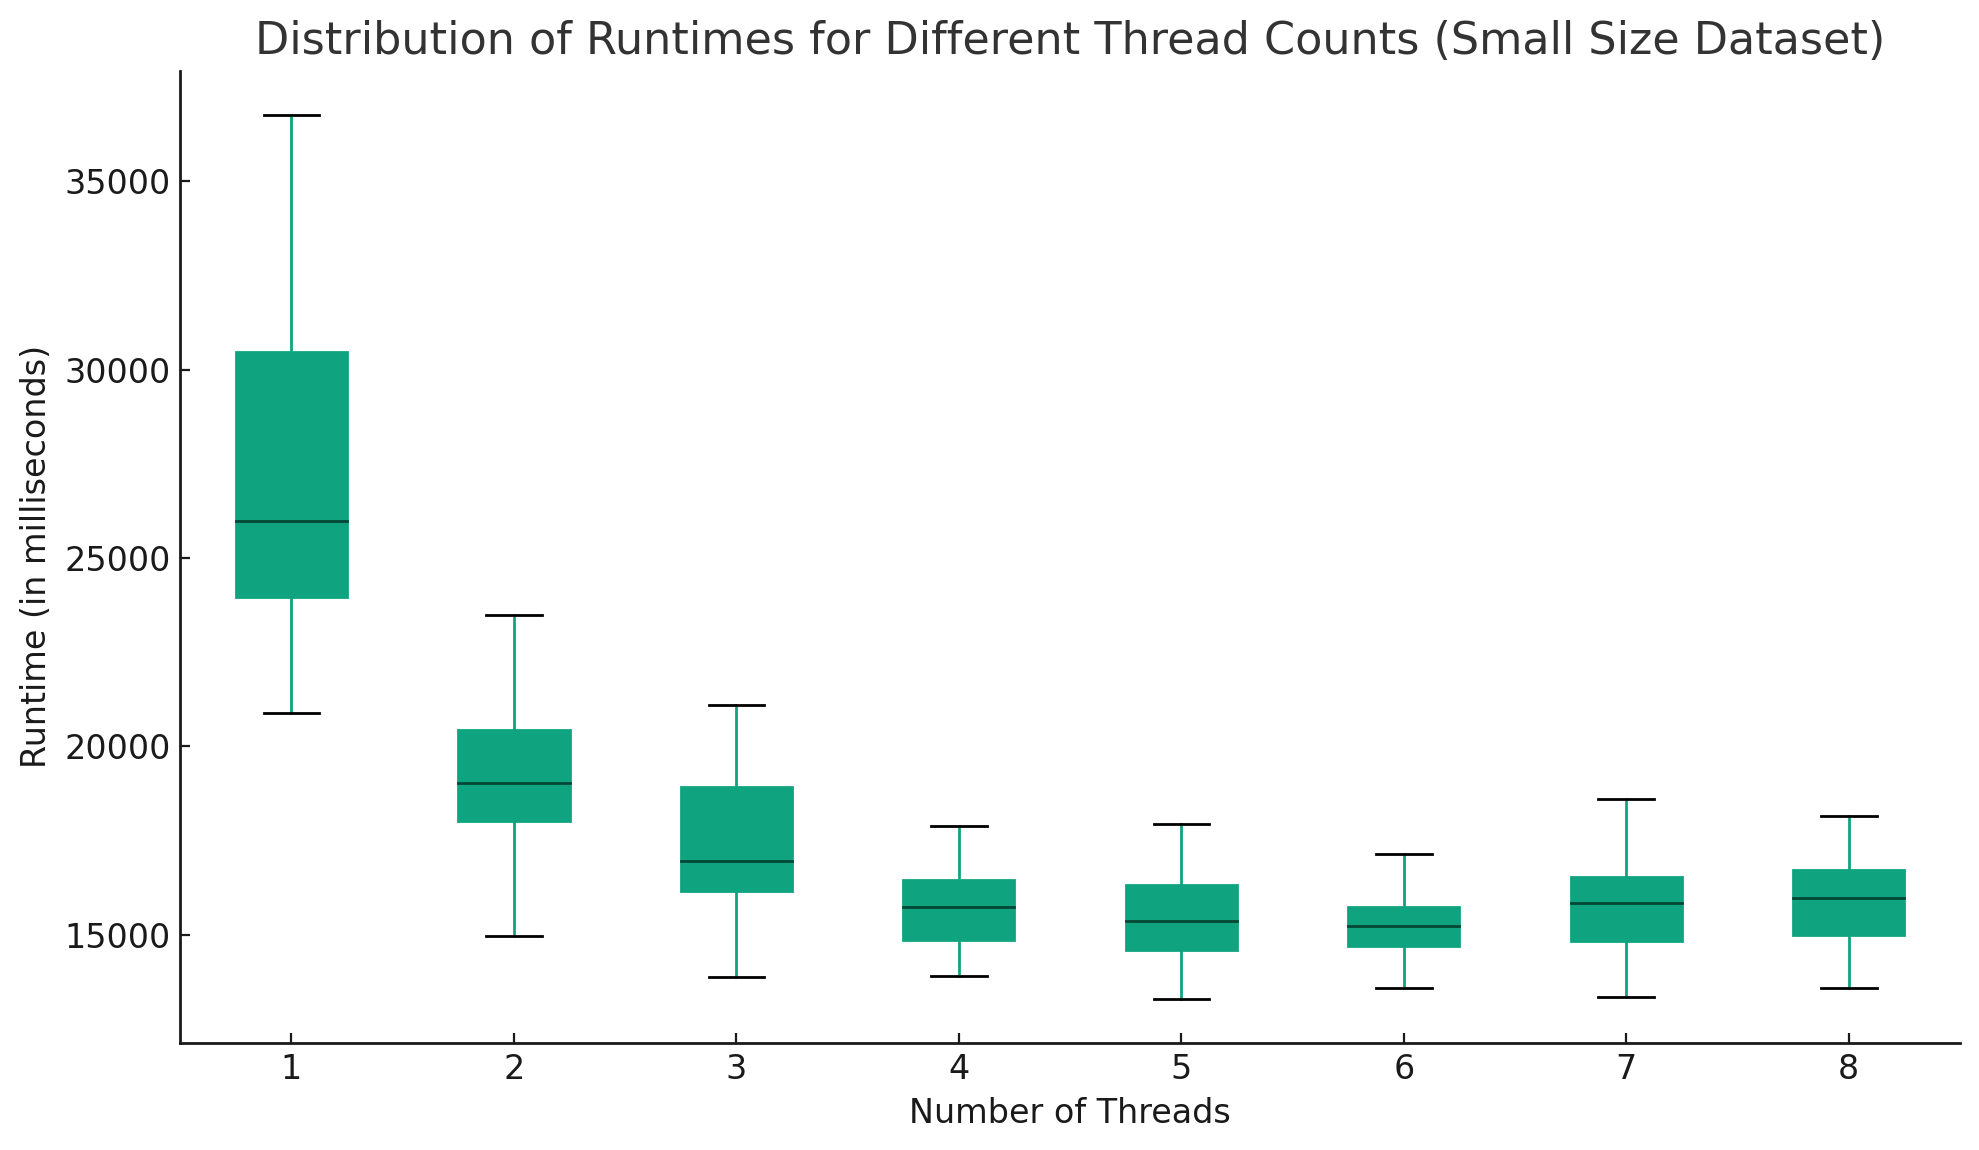
\includegraphics[scale=0.31]{boxplot_small.png}
    \end{figure}
\end{frame}

\begin{frame}{GRASP: Optimal Thread Count}
    \begin{itemize}
        \item Paired t-tests complemented the analysis.
        \item Visual inference suggests optimal thread count is 4 for both datasets.
    \end{itemize}
    \begin{figure}
        \centering
        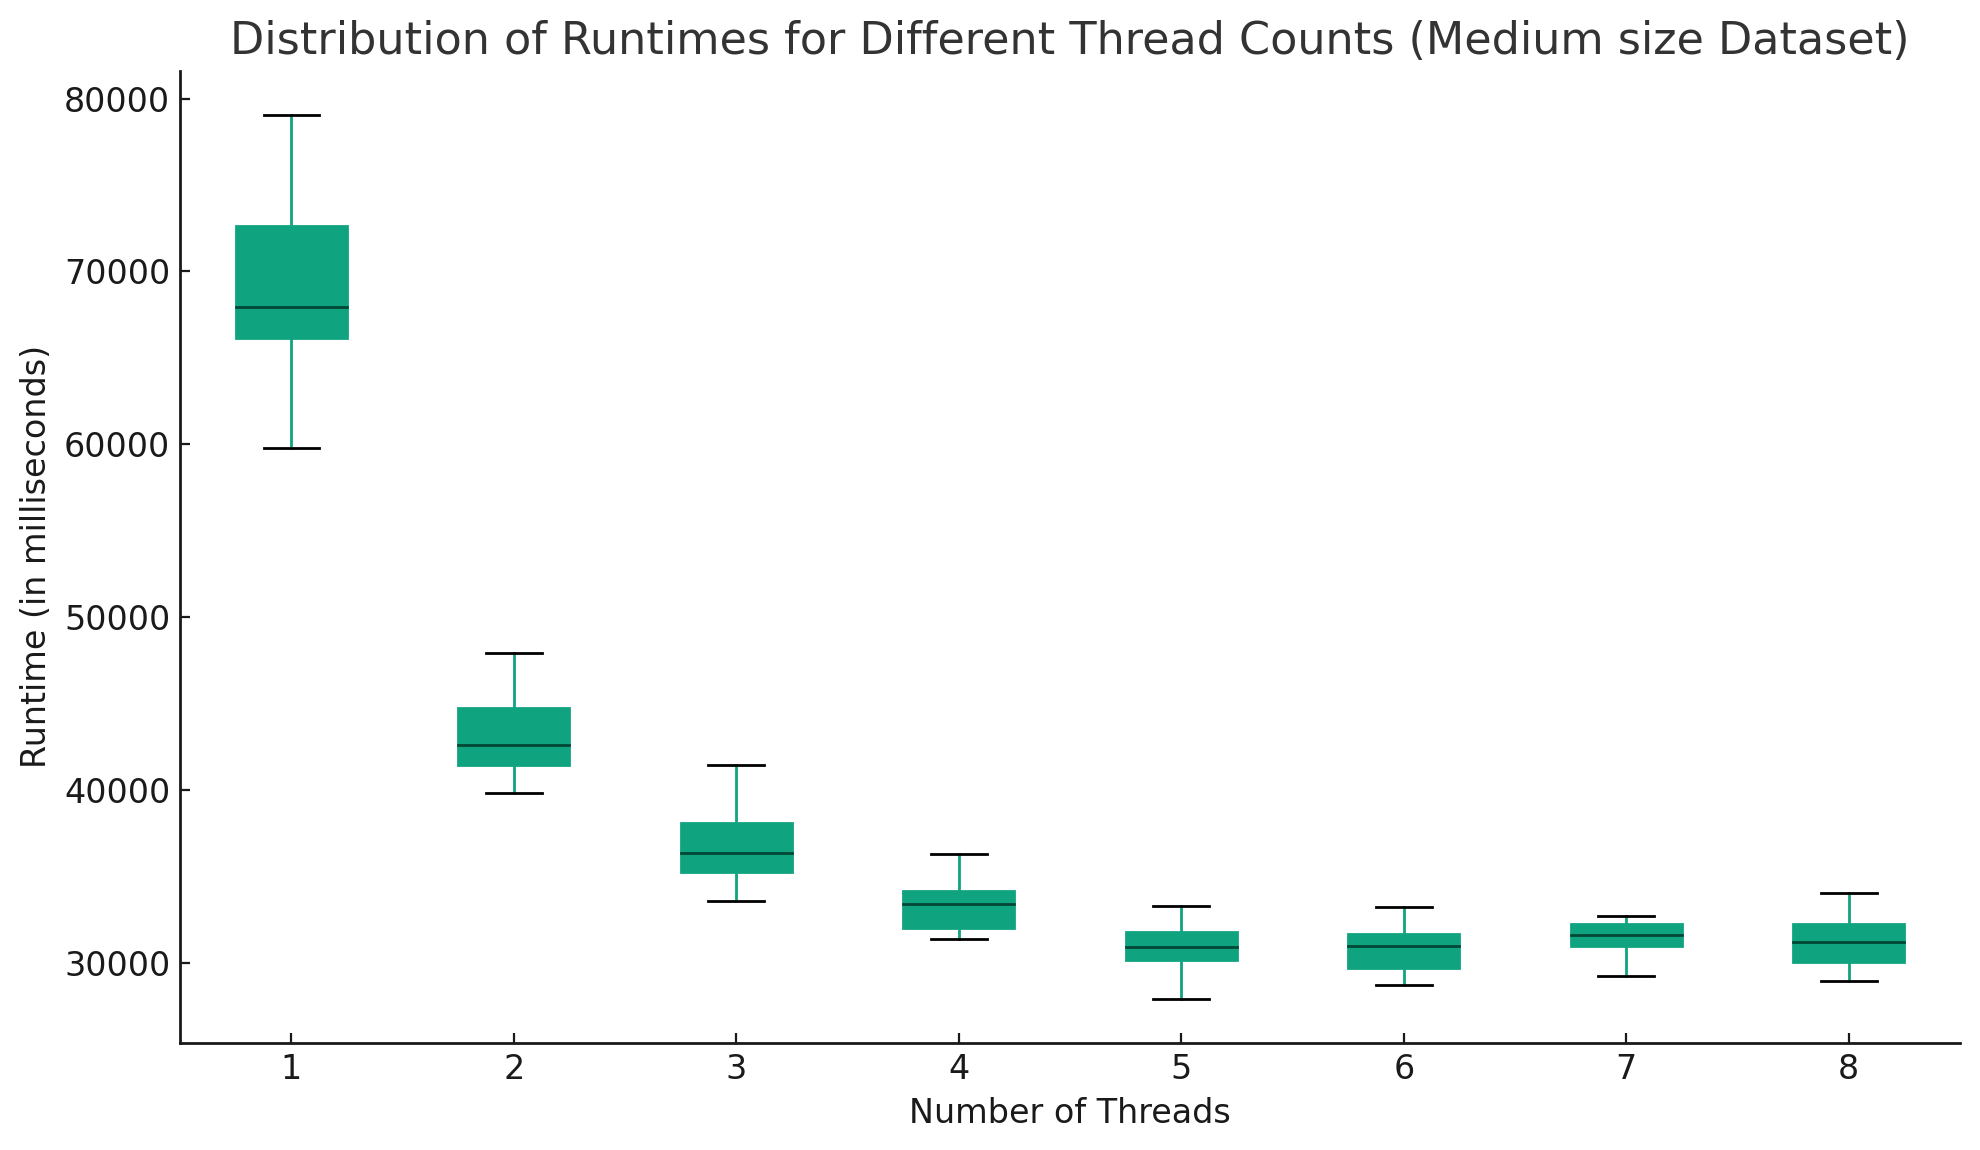
\includegraphics[scale=0.4]{boxplot_medium.png}
    \end{figure}
\end{frame}

\begin{frame}{GRASP: Calibration of Parameters}
    \begin{itemize}
        \item We explored calibration of 3 parameters: $\alpha_l, \alpha_a$, and \textit{max\_iters}.
        \item Tested combinations for subsets of Datasets 1 and 2, totaling 125 configurations:
        \begin{itemize}
            \item $\alpha_l \in \{0.1, 0.3, 0.5, 0.7, 0.9\}$
            \item $\alpha_a \in \{0.1, 0.3, 0.5, 0.7, 0.9\}$
            \item \textit{max\_iters} $\in \{10, 30, 50, 70, 90\}$
        \end{itemize}
    \end{itemize}
\end{frame}

\begin{frame}{GRASP: Findings from Calibration}
    \begin{itemize}
        \item Factorial ANOVA and One Way ANOVA:
            \begin{itemize}
                \item $\alpha_l, \alpha_a$ showed minimal effect on the objective function and runtime.
                \item \textit{max\_iters} impacted both runtime and objective function.
            \end{itemize}
        \item Chose $\alpha_l = 0.1$, $\alpha_a = 0.3$ for best mean runtime.
        \item Increasing \textit{max\_iters} from 10 to 90: 
            \begin{itemize}
                \item Improved objective function by ~1.541\%.
                \item Increased runtime by ~717.689\%.
            \end{itemize}
        \item Opted for \textit{max\_iters} = 70 for a balance of runtime and solution quality.
    \end{itemize}
    \small Note: The full results table isn't shown due to size constraints.
\end{frame}

\begin{frame}{GRASP Results}
    \begin{table}[h]
    \centering
    \scalebox{0.8}{
    \begin{tabular}{|c|c|c|c|}
        \hline
        \textbf{Dataset} & \textbf{GRASP Time} & \textbf{Gurobi Time} & \textbf{\%Rel diff. to Gurobi UB} \\
        \hline
        1 & 17.05 s & 1800 s & 2.88 \\
        \hline
        2 & 62 s & 1800 s & 5.23 \\
        \hline
        3 & 160 s & 7200 s & 7.91 \\
        \hline
    \end{tabular}
    }
    \caption{Comparison of Average values of Fine-tuned GRASP with 4 threads vs Gurobi}
    \label{tab:comparison}
\end{table}

\end{frame}

\section{Wrap-up}

\begin{frame}{Wrap-up}
    \small \textbf{Conclusions}
    \scriptsize
    \begin{itemize}
        \item $p$-dispersion heuristic for location and opportunity cost with the usage of efficient data structures for allocation offer the best performance in feasibility and speed.
        \item Fine-tuning GRASP: \textit{max\_iters}= 70, $\alpha_l = 0.1, \alpha_a = 0.3$ and 4 threads balances runtime and solution quality.
        \item GRASP's solutions closely rival Gurobi's but are significantly faster. For Dataset 1, GRASP outperformed Gurobi in several instances.
    \end{itemize}
    \small \textbf{Future work}
    \scriptsize
    \begin{itemize}
        \item Explore risk as an uncertainty measure.
        \item Introduce contiguity constraints.
        \item Hybridize with exact formulation.
        \item Investigate other strategies (TS, ILS, IGLS, VNS, SS).
    \end{itemize}
\end{frame}


\begin{frame}{Acknowledgments}
    \begin{itemize}
        \item Thank you very much for your attention!
        \item Feedback is welcome :)
        \item Email: eduardosalaz@outlook.com
        \item GitHub: \url{https://github.com/eduardosalaz}
    \end{itemize}
    
    \begin{figure}
        \centering
        
\includegraphics[scale=0.2]{uanl-logo}
        
\includegraphics[scale=0.2]{fime-logo}
    \end{figure}
\end{frame}

\begin{frame}{References}
\scalebox{0.8}{
\begin{minipage}{1.1\linewidth}
\printbibliography
\end{minipage}
}

\end{frame}
\end{document}